\chapter{هندسهٔ هزینه و هم‌راستایی آشفتگی}
\label{ch:geometry}

\section{از شکست حملهٔ تک‌گامی تا تفسیر هندسی}
\label{sec:geometry-motivation}

آموزش هم‌آورد، ستبری مدل دسته‌بندی را از راه یادگیری روی ورودی‌هایی دنبال می‌کند که هزینه را افزایش می‌دهند. ستبری، که در بخشی از ادبیات فارسی با تعبیر مقاوم بودن مدل نیز بیان می‌شود، به عملکرد در برابر مجموعه‌ای از تغییرات مجاز مربوط است؛ بنابراین موفقیت در برابر یک مولد مشخص نمونه، به‌تنهایی بیانگر ستبری نیست. در صورت‌بندی کمینه‌سازی و بیشینه‌سازی، کیفیت پاسخ تقریبی مسئلهٔ درونی مستقیماً بر معنای آموزشی مسئلهٔ بیرونی اثر می‌گذارد \cite{madry2018towards}. اگر حمله نقاط پرهزینه را پیدا نکند، کاهش هزینهٔ آموزشی ممکن است همراه با باقی ماندن آسیب‌پذیری در همان همسایگی باشد. این تمایز در آموزش سریع اهمیت بیشتری دارد، زیرا یک گام مبتنی بر شیب تنها تصویری محلی از هندسهٔ هزینه در اختیار دارد.

برای ورودی $x\in\IR^d$، برچسب $y$ و پارامترهای $\theta$، در این فصل از نگارش کوتاه
\begin{equation}
\ell_\theta(z)=\mathcal{L}(f_\theta(z),y),\qquad
g(z)=\nabla_z\ell_\theta(z)
\label{eq:geometry-loss}
\end{equation}
استفاده می‌شود. در هر تحلیل محلی، $y$ و $\theta$ ثابت‌اند. روش علامت شیب سریع، یعنی \lr{FGSM}، از تقریب خطی هزینه و جهت $\operatorname{sign}(g(x))$ استفاده می‌کند \cite{goodfellow2015explaining}. این جهت برای بیشینه‌سازی جملهٔ خطی روی کرهٔ $\ell_\infty$ مناسب است، اما دربارهٔ تغییر شیب در طول مسیر اطلاعاتی ندارد. شروع تصادفی در آموزش سریع، تنوع نقاط آغاز را افزایش می‌دهد، ولی اعتبار تقریب خطی را برای هر اندازهٔ گام تضمین نمی‌کند \cite{wong2020fast}.

بیش‌برازش فاجعه‌آمیز، با نماد \lr{CO}، زمانی مشاهده می‌شود که درستی در برابر حملات چندگامی به‌سرعت فرو می‌ریزد، در حالی که درستی در برابر حملهٔ تک‌گامی بالا می‌ماند یا افزایش می‌یابد. در این وضعیت، افزایش درستی تک‌گامی می‌تواند نشانهٔ ضعیف شدن مولد حمله باشد. مقالهٔ \sora{} این مسئله را با بررسی تغییر شکل سطح هزینه و مرز تصمیم تحلیل می‌کند \cite{sora2026}. شکل~\ref{fig:geometry-evolution} نشان می‌دهد که حتی پیش از خطای آشکار دسته‌بندی، مرز تصمیم می‌تواند پیرامون نقاطی که حملهٔ آموزشی به آن‌ها می‌رسد پیچ بخورد. حملهٔ چندگامی با تغییر متوالی جهت، ناحیهٔ آسیب‌پذیر بین این نقاط را پیدا می‌کند، در حالی که حملهٔ تک‌گامی از آن عبور می‌کند.

% Source: sora2026 paper Figure 1; already in paper; reproduced to explain the published geometric interpretation, not a new experiment.
\begin{figure}[tbp]
\centering
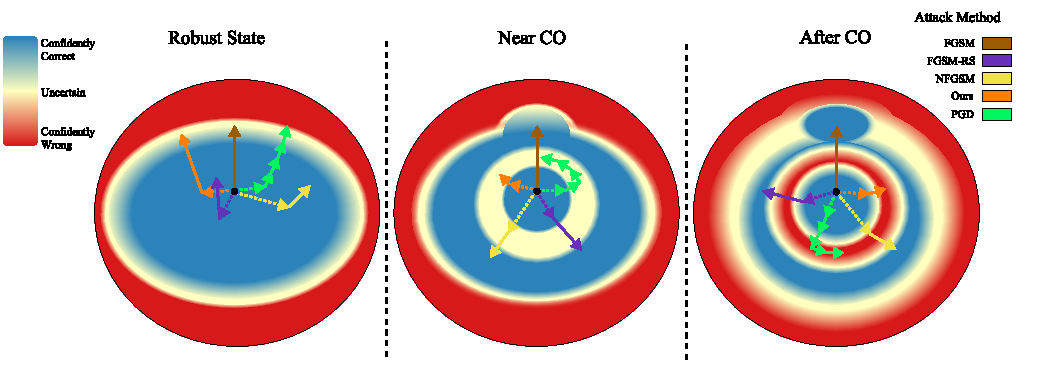
\includegraphics[width=\textwidth]{images/paper_geometry.pdf}
\caption[تحول هندسه هزینه پیش و پس از بیش‌برازش فاجعه‌بار]{تحول هندسهٔ هزینه در آموزش با \lr{FGSM}: از همسایگی تقریباً خطی در سمت چپ، به پیچش مرز تصمیم پیش از فروپاشی در میانه و ناحیهٔ قابل بهره‌برداری برای حملهٔ چندگامی در سمت راست. شکل، تفسیر هندسی گزارش‌شده در مقاله است و تضمینی دربارهٔ همهٔ ورودی‌ها ارائه نمی‌کند. بازنشر از شکل ۱ مقالهٔ \sora{} \cite{sora2026}.}
\label{fig:geometry-evolution}
\end{figure}

\section{بیش‌برازش به اندازهٔ آشفتگی}
\label{sec:geometry-eo}

\begin{تعریف}[بیش‌برازش اپسیلون]
بیش‌برازش اپسیلون، با نماد \lr{EO}، به الگوی یادگیری‌ای گفته می‌شود که در آن مدل در برابر آشفتگی‌های تولیدشده با اندازه‌های خاص، به‌ویژه اندازهٔ ثابت مورد استفاده در آموزش، عملکرد مناسبی دارد، اما در برابر اندازه‌های دیگر در همان جهت یا همسایگی، آسیب‌پذیر است. در تفسیر مقالهٔ \sora{}، تمرکز توزیع حمله روی دامنه‌ای محدود از اندازه و جهت، زمینهٔ این رفتار را فراهم می‌کند \cite{sora2026}.
\end{تعریف}

برای روشن شدن این مفهوم، جهت $p=\operatorname{sign}(g(x))$ را ثابت و تابع تک‌متغیرهٔ $\phi(t)=\ell_\theta(x+tp)$ را در نظر می‌گیریم. اگر تقریب خطی در بازهٔ مورد نظر معتبر باشد، انتظار می‌رود افزایش کوچک $t$ در جهت صعود، هزینه را افزایش دهد. اما $\phi$ ممکن است ابتدا افزایش یابد و سپس پیش از رسیدن به اندازهٔ آموزشی کاهش پیدا کند. در این حالت، مدل می‌تواند نقاط انتهایی مورد استفاده در آموزش را کم‌هزینه کند، در حالی که نقاط میانی پرهزینه باقی می‌مانند. مشاهدهٔ هزینهٔ کم در انتهای گام، اطلاعات کافی دربارهٔ کل پاره‌خط یا کل کرهٔ آشفتگی نمی‌دهد.

شکل~\ref{fig:geometry-epsilon} این مسئله را با تغییر اندازهٔ حمله نشان می‌دهد. در مدل دچار فروپاشی، درستی \lr{FGSM} نسبت به اندازهٔ گام رفتاری شدیداً نامونوا دارد. مقادیر منفی روی محور، حرکت در خلاف جهت ثابت انتخاب‌شده را نمایش می‌دهند؛ این مقادیر به معنای منفی بودن شعاع مجموعهٔ تهدید نیستند. برای بیشینه‌سازی دقیق روی مجموعه‌های تو‌در‌تو، بزرگ‌تر شدن شعاع نمی‌تواند بهترین هزینهٔ قابل دستیابی را کاهش دهد. نامونوا بودن منحنی حملهٔ تک‌گامی با این واقعیت تناقض ندارد، زیرا هر نقطهٔ منحنی حاصل یک حملهٔ تقریبی است، نه حل دقیق مسئلهٔ بیشینه‌سازی.

% Source: sora2026 paper Figure 2; already in paper; reproduced attack-strength sweep, with signed steps distinguished from threat radii.
\begin{figure}[tbp]
\centering
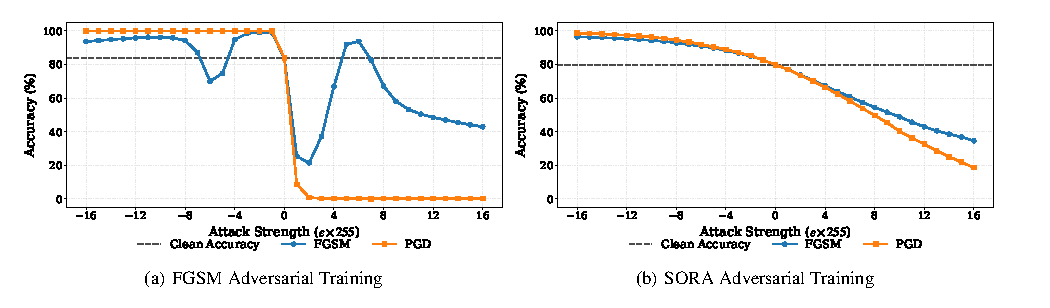
\includegraphics[width=\textwidth]{images/paper_epsilon.pdf}
\caption[درستی در برابر تغییر اندازه حمله و بیش‌برازش اپسیلون]{درستی در برابر تغییر اندازهٔ حمله برای مدل دچار بیش‌برازش فاجعه‌آمیز و مدل آموزش‌دیده با \sora{}. قله‌های درستی تک‌گامی در سمت چپ بیانگر محافظت یکنواخت در همسایگی نیستند. مقادیر منفی محور افقی ضریب حرکت در خلاف جهت حمله‌اند. بازنشر از شکل ۲ مقالهٔ \sora{} \cite{sora2026}.}
\label{fig:geometry-epsilon}
\end{figure}

این تفسیر، بیش‌برازش اپسیلون را به تنوع مولد حمله مرتبط می‌کند. شروع تصادفی نقطهٔ ارزیابی شیب را جابه‌جا می‌کند و تصادفی کردن دامنه، نقاط متفاوتی در طول جهت‌های انتخاب‌شده می‌سازد. در مقابل، تکرار یک اندازهٔ ثابت ممکن است به مدل اجازه دهد تنها نواحی پرتکرار را ترمیم کند. با این حال، افزودن نویز به‌تنهایی تضمین نمی‌کند که نقاط پرهزینه نمونه‌برداری شوند. بزرگی نویز، برش نهایی و ساختار دادگان بر توزیع مؤثر نمونه‌های آموزشی اثر دارند. از این رو، توضیح هندسی باید همراه با مشخص کردن مولد واقعی آشفتگی به کار رود.

بیش‌برازش اپسیلون و بیش‌برازش فاجعه‌آمیز دو تعبیر هم‌ارز ریاضی نیستند. اولی به حساسیت نسبت به اندازه و مسیر حمله اشاره دارد و دومی با افت ناگهانی ستبری ارزیابی‌شده شناخته می‌شود. شواهد مقاله رابطهٔ نزدیکی میان آن‌ها نشان می‌دهد، ولی قضیه‌ای که وجود یکی را برای همهٔ شبکه‌ها شرط لازم و کافی دیگری بداند ارائه نمی‌کند. کاربرد این دیدگاه، توضیح یک سازوکار محتمل و طراحی نشانه‌های پایش است؛ تشخیص نهایی ستبری همچنان به حملات ارزیابی مناسب وابسته می‌ماند.

\subsection{نمونه‌های هم‌آورد غیرعادی}
\label{sec:geometry-aae}

\begin{تعریف}[نمونهٔ هم‌آورد غیرعادی]
برای نقطهٔ مبنای $z$ و گام حملهٔ $\delta$، اگر
\begin{equation}
\ell_\theta(z+\delta)<\ell_\theta(z),
\label{eq:geometry-aae}
\end{equation}
برقرار باشد، خروجی حمله نسبت به این مبنا یک نمونهٔ هم‌آورد غیرعادی، با نماد \lr{AAE}، نامیده می‌شود. در حالت شروع تصادفی، مبنای مقایسه می‌تواند $z=x+\eta$ باشد؛ مقایسه با ورودی پاک $x$ باید جداگانه مشخص شود \cite{lin2023eliminating,sora2026}.
\end{تعریف}

واژهٔ غیرعادی به شکست هدف افزایش هزینه اشاره دارد. این تعریف مستلزم آن نیست که نمونهٔ نهایی حتماً درست دسته‌بندی شود یا نمونهٔ مبنا حتماً خطا داشته باشد؛ هزینهٔ پیوسته و برچسب پیش‌بینی‌شده دو کمیت متفاوت‌اند. همچنین حمله‌ای که هزینه را اندکی افزایش داده است می‌تواند هنوز بسیار ضعیف‌تر از حملهٔ چندگامی باشد. بنابراین سهم پایین نمونه‌های غیرعادی شرط کافی برای کیفیت مولد حمله نیست.

در هندسهٔ دارای قله و فرورفتگی، گام بلند می‌تواند از ناحیهٔ پرهزینه عبور کند و در نقطه‌ای کم‌هزینه پایان یابد. آموزش روی این نقاط ممکن است نواحی از پیش کم‌هزینه را بیشتر تقویت کند و ناحیهٔ آسیب‌پذیر میانی را دست‌نخورده بگذارد. این سازوکار، افزایش ظاهراً مطلوب درستی \lr{FGSM} را توضیح می‌دهد. نرخ نمونه‌های غیرعادی نشانه‌ای قابل استفاده است، ولی ممکن است پس از شروع تغییر هندسه افزایش یابد. مقاله با همین انگیزه، مقایسهٔ شیب در دو سر گام را برای تشخیص زودتر تغییر مسیر هزینه پیشنهاد می‌کند \cite{sora2026}.

\section{تعریف و محاسبهٔ هم‌راستایی آشفتگی}
\label{sec:geometry-pertalign}

\begin{تعریف}[هم‌راستایی آشفتگی]
نقطهٔ آغاز حمله را $z=x+\eta$، جهت ثابت گام را $v$ و اندازهٔ اسکالر آن را $\alpha$ می‌گیریم. برای دو شیب ناصفر $g=\nabla\ell_\theta(z)$ و $g'=\nabla\ell_\theta(z+\alpha v)$، معیار \pertalign{} برابر است با
\begin{equation}
P(z,v,\alpha)=\frac{g^{\mathsf T}g'}{\|g\|_2\|g'\|_2}.
\label{eq:geometry-pertalign}
\end{equation}
شروع تصادفی مقاله از توزیع $\eta\sim\mathcal{U}([-\epsilon,\epsilon]^d)$ انتخاب می‌شود و جهت متداول، $v=\operatorname{sign}(g)$ است \cite{sora2026}.
\end{تعریف}

این معیار زاویهٔ میان شیب آغاز و پایان گام را اندازه می‌گیرد. مقدار نزدیک یک به معنای حفظ جهت شیب در دو نقطه است، مقدار نزدیک صفر بیانگر تقریباً عمود شدن آن‌ها و مقدار منفی بیانگر چرخش بیش از زاویهٔ قائمه است. چون اندازهٔ شیب در مخرج حذف می‌شود، افزایش یا کاهش شدید اندازه می‌تواند پشت هم‌راستایی زیاد پنهان بماند. در عمل، حفاظت عددی از مخرج برای شیب‌های کوچک ضروری است؛ مقدار حاصل از چنین حفاظتی نباید مانند کسینوس دقیق تفسیر شود.

مزیت محاسباتی معیار از محل دسترسی به دو شیب می‌آید. شیب اول برای ساخت حمله لازم است. در گذر پس‌رو روی نمونهٔ هم‌آورد، علاوه بر مشتق پارامترها می‌توان مشتق هزینه نسبت به ورودی هم‌آورد را نیز دریافت کرد. این مشتق دوم با امتداد همان گذر تا ورودی به دست می‌آید و به حملهٔ تکراری جداگانه نیاز ندارد. این تعبیر، هزینهٔ ناچیز را نسبت به آموزش تک‌گامی توضیح می‌دهد؛ محاسبهٔ ضرب داخلی و نگهداری آرایهٔ شیب همچنان هزینهٔ محدود خود را دارند.

% Source: sora2026 paper Figure 3; already in paper; reproduced published monitoring curves, not independently measured thesis results.
\begin{figure}[tbp]
\centering
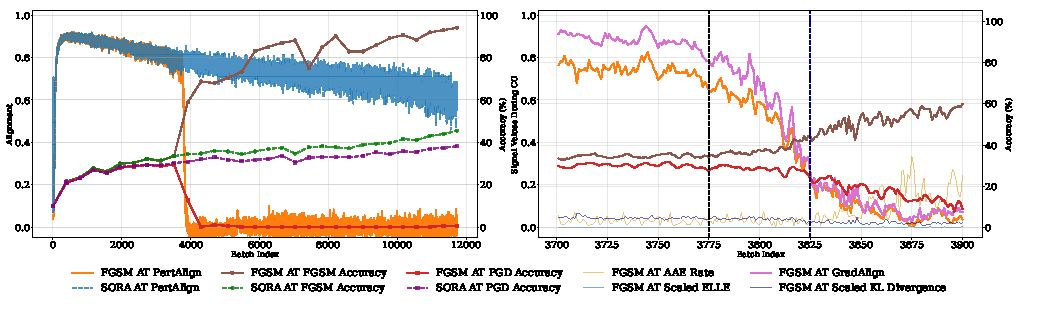
\includegraphics[width=\textwidth]{images/paper_pertalign.pdf}
\caption[پایش هم‌راستایی آشفتگی و هشدار پیش از فروپاشی]{پایش \pertalign{} در آزمایش گزارش‌شده روی \lr{CIFAR-10}. در بزرگ‌نمایی سمت راست، افت معیارهای هم‌راستایی پیش از جدایی آشکار درستی تک‌گامی و چندگامی دیده می‌شود. تقدم زمانی در این نمودار یک مشاهدهٔ تجربی است و زمان هشدار ثابتی برای همهٔ تنظیمات تضمین نمی‌کند. بازنشر از شکل ۳ مقالهٔ \sora{} \cite{sora2026}.}
\label{fig:geometry-pertalign}
\end{figure}

\section{رابطهٔ محلی با هسین}
\label{sec:geometry-hessian}

\begin{لم}[بخش عمود کنش هسین]
\label{lem:geometry-projected-hessian}
فرض کنید هزینه در همسایگی $z$ هموار، هسین آن محلی لیپشیتس و $g\ne0$ باشد. جهت $v$ هنگام تحلیل ثابت است. با تعریف $H=\nabla^2\ell_\theta(z)$، $\widehat g=g/\|g\|_2$ و تصویر متعامد $Q_g=I-\widehat g\widehat g^{\mathsf T}$، برای $\alpha$ به‌اندازهٔ کافی کوچک داریم
\begin{equation}
1-P(z,v,\alpha)
=\frac{\alpha^2}{2\|g\|_2^2}\|Q_gHv\|_2^2+O(\alpha^3).
\label{eq:geometry-projected-hessian}
\end{equation}
این بیان، صورت تصویری رابطهٔ نظری پیوست الف مقاله است \cite{sora2026}.
\end{لم}

\begin{اثبات}
بسط شیب در امتداد جهت ثابت می‌دهد
\begin{equation}
g'=g+\alpha Hv+R,\qquad \|R\|_2=O(\alpha^2).
\label{eq:geometry-gradient-expansion}
\end{equation}
اگر $k=g^{\mathsf T}Hv/\|g\|_2^2$ و $\gamma=g^{\mathsf T}R/\|g\|_2^2$ باشد، صورت و مخرج کسینوس پس از تقسیم بر $\|g\|_2^2$ به شکل
\begin{equation}
P=\frac{1+\alpha k+\gamma}
{\sqrt{1+2\alpha k+2\gamma+
\alpha^2\|Hv\|_2^2/\|g\|_2^2+O(\alpha^3)}}
\end{equation}
درمی‌آیند. بسط ریشه و معکوس آن نشان می‌دهد که جمله‌های مرتبهٔ اول و سهم مشترک $\gamma$ حذف می‌شوند و
\begin{equation}
P=1-\frac{\alpha^2}{2}
\left(\frac{\|Hv\|_2^2}{\|g\|_2^2}-k^2\right)+O(\alpha^3).
\end{equation}
عبارت داخل پرانتز برابر $\|Q_gHv\|_2^2/\|g\|_2^2$ است، زیرا $Q_g$ مؤلفهٔ موازی $g$ را حذف می‌کند. جایگذاری این همانی، نتیجه را می‌دهد.
\end{اثبات}

جهت حمله ممکن است از $g(z)$ ساخته شده باشد، ولی در این بسط مقدار محاسبه‌شدهٔ آن ثابت نگه داشته می‌شود. مشتق‌گیری از خود الگوریتم تولید جهت، مسئلهٔ دیگری است. افزودن شروع تصادفی نیز تنها نقطهٔ بسط را تغییر می‌دهد؛ فرض همواری باید پیرامون همان نقطه برقرار باشد. در شبکه‌های دارای فعال‌ساز تکه‌ای، عبور از مرز نواحی هموار می‌تواند اعتبار باقی‌ماندهٔ تیلور را محدود کند. بنابراین رابطهٔ بالا یک توصیف محلی از هزینه است و برای گام‌های بزرگ، بدون بررسی اضافی قابل تعمیم نیست.

\subsection{چه چیزی از هم‌راستایی زیاد نتیجه نمی‌شود؟}
\label{sec:geometry-limits}

رابطهٔ \eqref{eq:geometry-projected-hessian} فقط به بخش عمود $Hv$ حساس است. نزدیک بودن \pertalign{} به یک به معنای کوچک بودن نرم هسین، کم بودن همهٔ خمیدگی‌ها یا خطی بودن هزینه نیست. حتی استنتاج کوچک بودن بخش عمود نیز به اندازهٔ گام، اندازهٔ شیب و معتبر بودن تقریب وابسته است؛ گام بسیار کوچک می‌تواند در یک سطح پرخمیدگی هم کسینوسی نزدیک یک ایجاد کند. در مثال درجه‌دو با $H=MI$، جهت $v=g$ و $M>0$، رابطهٔ $g'=(1+\alpha M)g$ برقرار است. در نتیجه $P=1$، در حالی که $\|H\|_2=M$ می‌تواند به دلخواه بزرگ باشد.

برای $v=g$، شرط حذف جملهٔ اصلی ناهم‌راستایی به صورت $Hg=kg$ نوشته می‌شود: شیب در یک جهت ویژهٔ هسین قرار گرفته است. مقدار ویژهٔ $k$ لزوماً کوچک نیست. همچنین کران بالایی بر ناهم‌راستایی برحسب نرم هسین، استنتاج معکوس دربارهٔ کوچک بودن هسین را مجاز نمی‌کند. برای $v=\operatorname{sign}(g)$ نیز موضوع، کنش هسین روی جهت علامت است؛ نمی‌توان فرمول ویژهٔ جهت شیب را بی‌تغییر به آن نسبت داد.

تعبیر نیوتنی به احتیاط دیگری نیاز دارد. شرط $Hv=cg$ برای هسین وارون‌پذیر، $v=cH^{-1}g$ را نتیجه می‌دهد؛ اما برای هسین تکین، اگر $c\ne0$ و معادله سازگار باشد، پاسخ کلی برابر است با
\begin{equation}
v=cH^\dagger g+w,\qquad w\in\ker H,
\label{eq:geometry-pseudoinverse}
\end{equation}
و سازگاری مستلزم $g\in\operatorname{range}(H)$ است. برای نمونه، با $H=\operatorname{diag}(1,0)$، $g=(1,0)^{\mathsf T}$ و $v=(1,1)^{\mathsf T}$، رابطهٔ $Hv=g$ برقرار است، ولی $v$ مضربی از $H^\dagger g=(1,0)^{\mathsf T}$ نیست. در حالت $c=0$ نیز هر جهت پوچ می‌تواند بخش عمود را صفر کند. از این رو، هم‌راستا بودن $Hv$ و $g$ به‌طور عمومی هم‌راستایی $v$ و شبه‌وارون هسین ضرب در شیب را ثابت نمی‌کند. افزون بر این، جهت نیوتنی فقط با بررسی علامت خمیدگی و مسئلهٔ بیشینه‌سازی معنای بهینگی پیدا می‌کند.

\section{مقایسه با هم‌راستایی شیب}
\label{sec:geometry-gradalign}

معیار \lr{GradAlign} کسینوس شیب در ورودی پاک و یک همسایهٔ تصادفی را بررسی می‌کند:
\begin{equation}
G(x,\eta)=\cos\!\left(\nabla\ell_\theta(x),\nabla\ell_\theta(x+\eta)\right),
\qquad \eta\sim\mathcal{U}([-\epsilon,\epsilon]^d).
\label{eq:geometry-gradalign}
\end{equation}
در روش اصلی، جملهٔ $1-G$ با ضریبی مشخص به هدف آموزشی افزوده می‌شود تا جهت شیب در همسایگی پایدارتر شود \cite{andriushchenko2020understanding}. در مقابل، \pertalign{} دو سر گام حمله را مقایسه می‌کند و به‌عنوان معیار پایش به کار می‌رود. در \sora{} این معیار مستقیماً به هزینه افزوده نمی‌شود؛ سازگارسازی گام از آمارهٔ دیگری استفاده می‌کند که در فصل~\ref{ch:method} معرفی می‌شود.

از دید هندسی، لم~\ref{lem:geometry-projected-hessian} برای جابه‌جایی تصادفی کوچک نیز قابل استفاده است. پس شباهت روند دو معیار دور از انتظار نیست، ولی جهت مشاهدهٔ آن‌ها متفاوت است: یکی همسایه‌ای تصادفی را می‌بیند و دیگری مسیر منتخب حمله را. هیچ‌یک نرم کامل هسین را اندازه نمی‌گیرند. پایین‌تر بودن یکی در یک آزمایش، حکم عمومی دربارهٔ تمام جهت‌های تصادفی یا هم‌آورد ایجاد نمی‌کند؛ این موضوع به هندسهٔ مدل و توزیع نقاط وابسته است.

تمایز محاسباتی به کاربرد معیار مربوط است. منظم‌سازی با \lr{GradAlign} مستلزم انتقال مشتق اثر معیار به پارامترهاست و می‌تواند مشتقات مرتبهٔ بالاتر و نگهداری گراف بیشتری بخواهد. محاسبهٔ صرف یک کسینوس به چنین هزینه‌ای نیاز ندارد. \pertalign{} برای گزارش و کنترل بیرونی حمله از شیب‌های موجود استفاده می‌کند و از خود کسینوس نسبت به پارامترها مشتق نمی‌گیرد. روش‌های مبتنی بر خطی‌بودن محلی، مانند \lr{ELLE}، نیز با نمونه‌برداری‌های دیگر نشانه‌های مکملی از شکل هزینه فراهم می‌کنند \cite{rocamora2024efficient}؛ یکسان دانستن همهٔ این نشانه‌ها تفاوت محل اندازه‌گیری و هزینهٔ استفادهٔ آموزشی را پنهان می‌کند.

شکل~\ref{fig:geometry-pertalign} شواهد مقاله برای امکان هشدار زودهنگام را نشان می‌دهد، اما آستانهٔ جهان‌شمول یا تضمین جلوگیری از فروپاشی از آن به دست نمی‌آید. میانگین یک دسته می‌تواند رفتار اقلیتی از ورودی‌ها را پنهان کند و تغییر اندازهٔ گام نیز خود مقدار معیار را تغییر می‌دهد. در نتیجه، تفسیر مناسب شامل بررسی روند هم‌راستایی در کنار درستی پاک، درستی چندگامی، اندازهٔ گام و سهم نمونه‌های غیرعادی است. این چارچوب زمینهٔ ساخت یک کنترل‌کنندهٔ کم‌هزینه برای حمله را فراهم می‌کند، بدون آنکه نقش ارزیابی مستقل ستبری را حذف کند.
